\chapter{Reward-based Charging Schedule for a Community-based Ride-sharing Service}
\label{chapter5}

The models presented in chapters 3 and 4 have set the path for the intended carbon-neutral, scalable and decentralised ride-sharing service. In particular, Chapter 3 has explored the use of RES by the SECs, and the impact different AEV release approaches (e.g., START vs. SPREAD) has in the amount of TPs being served. Likewise, Chapter 4 examined the inter-relation of SECs, and the impact their negotiation process for allocating the AEV fleet has in the collective amount of TPs being served. 

The increasing integration of AAEVs in ride-sharing services introduces several complexities, particularly around the effective scheduling of charging sessions to maintain uninterrupted service availability \cite{energydatamanagement}. Current solutions often fall short in managing these challenges, either due to a lack of scalability, inefficient charging coordination, or limited consideration of SEC dynamics \cite{boasso2021sec}. Therefore, this chapter expands the key features of carbon neutrality and SEC interrelation by designing, implementing and evaluating a reward-based, intelligent charging scheduling to be integrated to the ride-sharing service. 

The new model sees each SEC owning a number of Charging Stations (CSs), and it RES-generated energy being split into (i) the energy used to release its own AAEVs and (ii) the energy used to re-charge already operative AAEVs. The new model exploits the inter-relation of SECs, enabling (1) host TPs to be served by an AEV of a different SEC, and (2) such AAEVs to re-charge their batteries in a host CSs in return. This charging scheduler involves a sophisticated decision-making process that accounts for multiple factors critical to the sustainable operation of the ride-sharing service. These factors include the proximity and waiting times of available CSs, the potential for service interruptions due to charging, and the dynamic re-allocation of AAEVs based on real-time assessments of energy consumption and vehicle availability. Additionally, the algorithm incorporates the flexibility to modify charging schedules dynamically by considering the collective prospects of multiple AAEVs. Overall, the charging scheduler aims to increase the robustness of the ride-sharing service, maximising its service across the entire time horizon. 

As with previous models, the charging scheduler is evaluated by aligning existing benchmarks (i.e. Google HashCode) and public datasets (i.e. NYC taxis) to the proposed problem formulation, simulating a variety of operational scenarios.

The chapter is organised as follows: Section \ref{sec:problem_definition} formalises the problem and Section \ref{sec:solution_approach} details the solution approach. Next, Section 5.3 presents an overall evaluation, with sections 5.4 to 5.7 then focusing on specific aspects, such as a comparison with baseline algorithms, the impact of charging speed, RES availability and TPs flexibility.  Finally, Section \ref{sec:conclusions_and_future_work} presents the main conclusions.


\section{Problem Definition}
\label{sec:problem_definition}

This section formalises the problem for integrating a reward-based, intelligent charging scheduling to the ride-sharing service defined in chapters 3 and 4. The new model integrates passenger allocation and re-routing constraints as both the TPs and the number of available vehicles evolve during a simulated time horizon. Aligning with the original formulation from Chapter 3, the ride-sharing service aims to maximise the number of TPs served and is designed to be highly scalable for large cities.

To better discuss the problem, its main features are enumerated here again, together with the novel features for the charging scheduler:
\begin{itemize}
    \item The grid dimensions of the city $c_r$, $c_c$ and the time horizon for the simulation $th$.Manhattan distances among the locations of the city are assumed.
    \[
    (c_r, c_c, th)
    \]
    \item A set $S$ of SECs, each with an id $s_{id}$, a location in the city $s_x$, $s_y$, a lexicographically ordered list of the vehicles belonging to it $s_E$, and the number of vehicles ready at the start of the simulation $s_R$.
    \[
    (s_{id}, s_x, s_y, s_R) \forall s \in S
    \]
    \item A set $E$ of AEVs, each with an id $e_{id}$, the id of the SEC it belongs to $s_{id}$, and its battery and passenger capacities ($e_{bc}$ and $e_{pc}$). A mapping from $E$ to $S$ is assumed, such that each $e_{id}$ belongs to one $s_{id}$. All AEVs are available at the start of the simulation.
    \[
    (s_{id}, e_{id}, e_{bc}, e_{pc}) \forall e \in E
    \]
    \item A set $T$ of TPs (TPs), each with an id $t_{id}$, its pick-up and drop-off locations $t_{px}, t_{py}, t_{dx}, t_{dy}$, and time windows $t_{ep}, t_{lp}, t_{ed}, t_{ld}$. Each TP includes a weight parameter $t_{w}$ indicating the importance of the TP. $t_{sid}$ id of the SEC $t_{id}$ is originating from. 
    \[
    (t_{id}, t_{px}, t_{py}, t_{dx}, t_{dy}, t_{ep}, t_{lp}, t_{ed}, t_{ld}, t_{w}, t_{sid}) \forall t \in T
    \]
    \item A set of charging stations (CSs) within the SECs, each represented by:
    \[
    (cs_{id}, s_{id}, cs_x, cs_y, cs_k, cs_{bn}) \forall c \in \mathcal{C}
    \]
    where $cs_{id}$ is the charging station ID, $s_{id}$ is the SEC ID, $cs_x$ and $cs_y$ are the coordinates, $cs_k$ is the queue limit which is the maximum number of AEVs that can charge at a charging station at a given same time, and $cs_{bn}$ is the charging rate per unit time which is used to compute the charging duration of an EV.
\end{itemize}

\subsection{Constraints}

The problem involves several key constraints that ensure the system operates efficiently and meets its objectives.

\begin{enumerate}
    \item \textbf{Trip Allocation Constraints:} A TP $t_{id}$ is allocated to an EV $e_{id}$ if the vehicle can meet the time-windows and capacity requirements:
    \[
    (e_{pc} \geq t_w \wedge e_{bc} \geq \text{required energy})
    \]
    This constraint ensures that each EV can handle the passenger load and has sufficient battery capacity to complete the trip.

    \item \textbf{Charging Constraints:} An EV is directed to a charging station when its battery level falls below a threshold $\beta$ or is \textit{idle} for the charging duration:
    \[
    [(e_{bc} \leq \beta) \wedge (e_{pc} \equiv 0)] \vee (m_i(TL_i) \equiv \text{idle})
    \]
    This constraint ensures that AEVs maintain sufficient battery levels and utilise idle times effectively for charging.

    \item \textbf{Reward $I$:} To promote inter-community service efficiency, AEVs receive a reward for serving trip petitions ($TPs$) originating from neighbouring SECs. Specifically, the reward gained by an AEV $e_{id}$ from serving a neighbouring TP $t_{id}$ is equal to the corresponding TP weight $t_{w}$:

        \[
        I_{e_{id}} = \sum_{t \in \mathcal{T}_{\text{neighboring}}} t_{w}
        \]
        
    The inclusion of this reward mechanism enhances system-level coordination in the decentralised scheduling process. Although SECs are assumed to operate under a cooperative framework, individual AEVs act as distributed agents making local decisions based on limited information. In such settings, reward structures serve as an indirect incentive alignment tool, guiding vehicle-level decision-making toward globally beneficial behaviours.
    
    In practical terms, the reward $I$ is integrated into the scheduling algorithm as part of the decision-making process. When multiple trip options are available, AEVs evaluate potential assignments based not only on travel distance or timing constraints but also on accumulated reward potential, prioritising trips that strengthen inter-SEC collaboration.
    
    The reward system thus functions as a lightweight reinforcement mechanism that:
    
    \begin{itemize}
        \item Encourages AEVs to serve TPs beyond their home SECs, improving geographic service coverage.
        \item Increases the overall number of TPs served, particularly in scenarios where local SEC capacity alone is insufficient.
        \item Provides a scalable, decentralised means of improving system efficiency, even in cooperative, non-competitive environments.
    \end{itemize}
    
    While Chapter 4 assumes cooperative SEC behaviour, the dynamic, decentralised nature of vehicle operations still benefits from  reward mechanisms to align individual vehicle actions with broader service objectives.
\end{enumerate}

\subsection{Solution Representation}
The solution to the problem is represented by the same two sets Alloc and Sched as in Chapter 3.

\begin{itemize}
    \item A set $Alloc$, representing an allocation mapping from $T$ to $E$.
    \[
    \forall t \in T \text{ } Alloc[t_{id}] = 
    \begin{cases}
        e_{id},  \text{if }  t_{id} \text{ is allocated to } e_{id}\\
        -1,  \text{otherwise}
    \end{cases}
    \]
    \item A set $Sched$, representing a scheduling mapping from $E$ to its sequence of movements (in chronological order) over the entire time horizon.
    \[
    \forall e \in E \text{ } Sched[e_{id}] = (m_0, m_1, \ldots, m_{n-1})
    \]
    Each movement $m_i$ of a vehicle is represented the same way as in Chapter 3, with special novel movement tags for charging actions
    \begin{align*}
    m_i \equiv \{ (TA_i, TB_i, AX_i, AY_i, BX_i, BY_i, PS_i, \\
        PE_i, ES_i, EE_i, TL_i, LW_i, TD_i) \}
    \end{align*}
    with: 
    \begin{itemize}
        \item $TA_i$ (resp. $TB_i$) represent the start time (resp. end time) of $m_i$.
        \item $AX_i$ and $AY_i$ (resp. $BX_i$ and $BY_i$) represent the coordinates of the vehicle at the start (resp. end) of $m_i$.
        \item $PS_i$ (resp. $PE_i$) represents the number of passengers in the vehicle at the start time (resp. end time) of $m_i$.
        \item $ES_i$ (resp. $EE_i$) represents the battery left in the vehicle at the start time (resp. end time) of $m_i$.
        \item $TL_i$ represents a label to identify the purpose of the trip.
        \begin{itemize}
            \item A movement for picking-up (resp. dropping off) the passenger of $t_{id}$ is marked as $+t_{id}$ (resp. $-t_{id}$).
            \item A charging movement is marked as $charge$. $+charge$ indicates charging at a SEC and $-charge$ indicates the journey to the charging station.
            \item A waiting movement is marked $wait$ indicating the wait time at a CS prior to charging.
        \end{itemize}
        \item $LW_i$ represents the leeway of the movement, i.e., the maximum delay that could be applied to the movement while still accomplishing the intended action.
        \item $TD_i$ represents the movement duration.
    \end{itemize}
\end{itemize}

\section{Solution Approach}
\label{sec:solution_approach}

This section presents the solution approach for the ride-sharing service. It consists of the integration of a newly developed charging scheduling algorithm into the previously developed trip allocation and vehicle routing algorithm of Chapter 3. 

\subsection{Vehicle Routing Algorithm}
\label{vehicle-allocation-algorithm}
The TP allocation and vehicle routing of the ride-sharing services builds upon the reactive ride-sharing algorithm previously developed in Chapter 3. 

One novel aspect of the current model is its proactiveness, as the algorithm is aware of the full set of TPs arising over the simulated time horizon, enabling it to take all TPs into account for decision-making. This contrasts with the reactive nature of the original model presented in Chapter 3, which dynamically re-allocated and re-scheduled AEVs as each new TP was introduced. The proactive simulation algorithm prioritises serving TPs ($t_{id}$) with the highest trip weights ($t_w$) first. It iterates through each $e_{id}$ in the set of AEVs, attempting to allocate the trip to the vehicle by dynamically re-routing its schedule. Once a trip is successfully allocated to a vehicle, the search stops. If no vehicle can allocate the trip, the attempt is considered unsuccessful.

Algorithm 4 presents the pseudo-code for the vehicle allocation and routing of the ride-sharing service. The function `Allocate' is the same as in Algorithm 1 in Chapter 3, and is provided here again for clarity purposes. The `Proactive\_Simulation' represents the modification w.r.t. Algorithm 1 in Chapter 3.

\begin{algorithm}
\caption{Proactive Ride-sharing Algorithm}
\begin{algorithmic}
\Function{allocate}{$e$, $t$, $Alloc[t]$, $Sched[e]$}
    \State $is\_allocated \gets false$
    \State $m \equiv [ m_0, \ldots, m_{k-1} ] \gets copy(Sched[e])$
    \For{$i \in 0, \ldots, k-1$}
        \If{$pick\_up(m, t, i)$}
            \State $m \gets [ m_0, \ldots, m_i', m_{i+1}', \ldots, m_{r-1}' ]$
            \For{$j \in i+1, \ldots, r-1$}
                \If{$drop\_off(m, t, j)$}
                    \State $m \gets [ m_0, \ldots, m_j'', m_{j+1}'', \ldots, m_{w-1}'' ]$
                    \If{$ret\_sec(m, w-1)$}
                        \State $m \gets [ m_0, \ldots, m_{w-1}'', m_w'' ]$
                        \State $(Alloc[t], Sched[e]) \gets (e, m)$
                        \State $is\_allocated \gets true$
                    \EndIf
                    \State \textbf{break}
                \EndIf
            \EndFor
            \State \textbf{break}
        \EndIf
    \EndFor
    \Return $is\_allocated$
\EndFunction
\\ \hrulefill
\Function{proactive\_simulation}{$S$, $E$, $T$, $th$}
    \State $(Alloc, Sched) \gets init(S, E, T, th)$
    \For{$t \in sortedByTripWeight(T)$}
        \For{$e \in E$}
            \If{$allocate(e, t, Alloc[t], Sched[e])$}
                \State \textbf{break}
            \EndIf
        \EndFor
    \EndFor
    \Return $(Alloc, Sched)$
\EndFunction
\end{algorithmic}
\end{algorithm}

%%%%%%%%%%%%%%%%%%%%%%%%%%%%%%%%%%%%%%%%%%%%%
% Subsection Charging Scheduling Mechanism
%%%%%%%%%%%%%%%%%%%%%%%%%%%%%%%%%%%%%%%%%%%%%
\subsection{Vehicle Charging Algorithm}

To integrate EV charging into the ride-sharing service, the following process is adopted. 

\subsubsection{Initial Scheduling}

Let \( E \) be the set of AEVs and \( T \) be the set of TPs (TPs). The vehicle routing algorithm computes the initial schedules for all AEVs, denoted as \( S_e \) for each \( e \in E \). Each schedule \( S_e \) includes a sequence of movements \( m_i \) with associated pick-up and drop-off times \( TA_i \) and \( TB_i \), locations \( (AX_i, AY_i) \) and \( (BX_i, BY_i) \), battery levels \( ES_i \) and \( EE_i \), and other parameters, ensuring all time windows and capacity constraints are met.

\subsubsection{Optimal Charging Points}

Given the initial schedules \( S_e \), the vehicle charging algorithm identifies optimal charging points within the schedule of each EV based on several factors:

\begin{enumerate}
    \item \textbf{Current Battery Capacity:} Let \( \beta \) be the battery threshold. Prioritise AEVs with \( e_{bc} < \beta \).
    \[
    \text{Priority}(e) \propto \left( \frac{1}{e_{bc}} \right)
    \]
    
    \item \textbf{Incentives Earned:} Let \( I_{s_{id}} \) be the incentives accumulated by SEC \( s_{id} \). Incentives influence the charging priority:
    \[
    \text{Priority}(e) \propto I_{s_{id}} \text{ for } e \in s_E
    \]
    
    \item \textbf{Proximity to Charging Stations (CS):} Let \( d(e, cs) \) be the Manhattan distance between EV \( e \) and charging station \( cs \). AEVs closer to a CS are preferred:
    \[
    \text{Priority}(e, cs) \propto \left( \frac{1}{d(e, cs)} \right)
    \]
    
    \item \textbf{Future Trip Potential:} Let \( V_e(t) \) be the potential number of trips an EV \( e \) can serve from the time it finishes charging \( t \) to the end of the time horizon \( th \). This is estimated by running the ride-sharing algorithm for the remaining time units:
    \[
    V_e(t) = \sum_{i=t}^{th} \left( \text{Weight of trips served by } e \text{ at time } i \right)
    \]
\end{enumerate}

% \subsubsection{Reward Mechanism}

% Each time an EV \( e \) serves a petition \( t \) from a neighboring SEC, its home SEC \( s_{id} \) gains incentives \( I_{s_{id}} \). These incentives are used to reward AEVs for charging sessions, encouraging AEVs to serve neighboring SECs:
% \[
% I_{s_{id}} = \sum_{t \in T_{\text{neighboring}}} t_w
% \]

\subsubsection{Eviction Policy}
An EV \( e_1 \) currently charging at a CS can be evicted if a newly arriving EV \( e_2 \) demonstrates a higher potential to serve additional trip petitions once recharged. The motivation for incorporating this eviction policy is grounded in the system-wide objective of maximising TP satisfaction, particularly in scenarios with constrained charging infrastructure or limited renewable energy availability.

CSs within SECs operate as bottlenecks in the overall ride-sharing service. In dynamic environments with fluctuating trip demands and decentralised AEV operations, the static allocation of charging slots based solely on arrival time can lead to suboptimal outcomes. Specifically, low-priority or underutilised AEVs occupying CSs may inadvertently block vehicles with greater potential to fulfill trip petitions, undermining system efficiency.
Let \( \tau \) be the time unit and \( d_{\text{charge}} \) be the charging duration. The ride-sharing algorithm is run for \( e_1 \) from \( \tau + d_{\text{charge}} \) to \( th \) and for \( e_2 \) from \( \tau \) to \( th \). EV \( e_1 \) is evicted if:
\[
V_{e_2}(\tau + d_{\text{charge}}) > V_{e_1}(\tau + d_{\text{charge}})
\]
Figure \ref{fig:eviction_policy} shows how the vehicle routes are taken into account to compute the eviction policy. 
\begin{figure}[h]
  \vspace{-0.2cm}
  \centering
  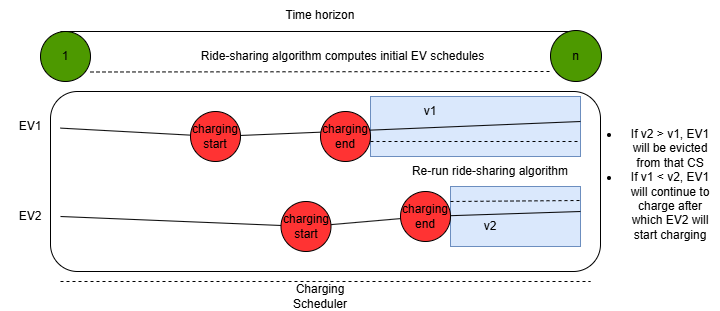
\includegraphics[width=7.5cm]{Crest/Images/eviction_policy.png}
  \caption{Eviction Policy}
  \label{fig:eviction_policy}
  \vspace{-0.1cm}
\end{figure}

\subsubsection{Iterative Process}

The vehicle charging algorithm iteratively refines battery re-charges for AEVs until no further improvements in the overall number of trips being served are observed. A maximum number of iterations \( n \) is given as input parameter. The follow 3-steps process is then performed until either the algorithm converges or reaches the maximum number of iterations.    %The process ensures optimal scheduling and resource utilisation:
\[
\text{Repeat until convergence:}
\begin{cases}
    \text{Run ride-sharing algorithm} \\
    \text{Update EV schedules} \\
    \text{Update charging decisions}
\end{cases}
\]
This iterative process aims for the overall system performance to continually improve, with the goal of maximising the number of TPs served while maintaining efficient resource allocation. Figure \ref{fig:flowchart} illustrates the interaction between the vehicle routing algorithm and the vehicle charging algorithm.
\begin{figure}[b]
  \vspace{-0.2cm}
  \centering
  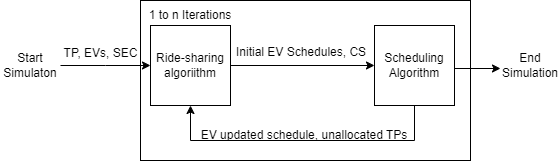
\includegraphics[width=7.5cm]{Crest/Images/flowchart.png}
  \caption{Interaction between Charging Scheduler and Ride-sharing Algorithms}
  \label{fig:flowchart}
  \vspace{-0.1cm}
\end{figure}

Algorithm 5 presents the pseudo-code for the vehicle charging of the ride-sharing service. Overall, key enhancements made to the ride-sharing service from its original implementation in Chapter 3 are:
\begin{itemize}
    \item Proactive scheduling to anticipate future TPs.
    \item Reward mechanisms to encourage strategic trip fulfillment.
    \item Strategic selection and management of CSs.
    \item Dynamic charging and eviction decisions based on potential trips being served.
    \item Iterative improvement processes to continually optimise system performance.
\end{itemize}

%%% Algorithm 2



\begin{algorithm}
\caption{Charging Scheduling Algorithm}
\begin{algorithmic}
\Function{Charging\_Scheduler}{$S$, $E$, $T$, $th$}

    \State $(Alloc, Sched) \gets init(S, E, T, th)$
    \State $X \gets \text{Sum  weights  TPs served in T } Alloc$
    \State $I_E \gets \text{sum  weights TPs served in neighboring SECs }$
    \State $no\_improvement\_count \gets 0$



    \While{$no\_improvement\_count < T$}
        \State $candidates \gets \text{FilterCandidates}(E, Sched)$
        \State $best\_candidate \gets \text{SelectBestCandidate}(candidates)$

        \If{$best\_candidate \neq \text{None}$}
            \State $\text{SendToCharge(best\_candidate)}$
            \State $sched \gets \text{RecomputeSchedule(best\_candidate.EV, Sched)}$
            \State $new\_X \gets \text{number of TPs being served in } Alloc$
            \If{$new\_X > X$}
                \State $X \gets new\_X$
                \State $no\_improvement\_count \gets 0$
            \Else
                \State $no\_improvement\_count \gets no\_improvement\_count + 1$
            \EndIf
        \Else
            \State $no\_improvement\_count \gets no\_improvement\_count + 1$
        \EndIf
    \EndWhile

    \Return $(Alloc, Sched)$
\EndFunction
\end{algorithmic}
\end{algorithm}

\section{Overall Evaluation}
\label{sec:evaluation}

This section assesses the charging scheduling algorithm proposed for a carbon-neutral, community-based, proactive ride-sharing service. The parameterised instance generator of Chapter 3 has been re-used to align existing benchmarks (i.e., Google Hashcode) and public datasets (i.e., NYC taxis) to the proposed problem formulation and to enable testing of the solution under various configurations.

\subsection{Experimental Setup}
The key parameters for the experiments are as follows:
\begin{enumerate}
    \item \textbf{Hashcode Dataset:} 10,000 TPs and 400 AEVs.
    \item \textbf{NYC Dataset:} 50,000 TPs and 1,000 AEVs.
\end{enumerate}

The key factors being explored are:
\begin{enumerate}
    \item \textbf{Number of SECs:} Different configurations of the number of SECs.
    \item \textbf{Energy Factor:} The energy available at each SEC.
    \item \textbf{Flexibility:} The flexibility in the pick-up and drop-off time windows of each TP.
\end{enumerate}

These factors lead to a wide range of results in terms of the overall number of trips being served, as shown in Table \ref{tab:datasets}. To analyse the charging algorithm, three instances of the Google Hashcode dataset are selected, as well as one instance of the New York City dataset to explore the scalability of the algorithm. 

The GHC dataset represents a synthetic, scalable benchmark environment specifically designed for algorithm stress-testing under controlled conditions. These controlled variations allow for a comprehensive sensitivity analysis of the proposed algorithms across different operational scenarios. In contrast, the NYC dataset represents a real-world, irregular urban topology derived from actual taxi trip data. Due to the inherent complexity, heterogeneity, and limited control over spatial and temporal patterns in this dataset, only one baseline configuration is applied. This configuration is selected to reflect a realistic, high-density urban mobility environment, providing a validity check for the proposed approach.

Table \ref{tab:datasets} shows the top results obtained from the \cite{smartgreens} ride-sharing solution where charging was not considered. 


\begin{table}[htbp]
\caption{Hashcode and NYC Instances}
\begin{center}
\begin{tabular}{|c|c|}
\hline
\textbf{Hashcode Instances Configuration}&\textbf{Trips Served}\\
\hline
GH01 Flexibility - 50\%; SECs - 16; Energy Factor - 2.0 & $\equiv$ 89.69\% \\
GH02 Flexibility - 25\%; SECs - 16; Energy Factor - 1.0 & $\equiv$ 51.19\% \\
GH03 Flexibility - 10\%; SECs - 1; Energy Factor - 2.0 & $\equiv$ 0.06\% \\
TPs = 10000, EV = 400 & \\
\hline
\textbf{NYC Instance Configuration}&\textbf{Trips Served}\\
\hline
NY01 Flexibility - 50\%; SECs - 16; Energy Factor - 2.0 & $\equiv$ 88.5\% \\
TPs = 50000, EV = 1000 & \\
\hline
\end{tabular}
\label{tab:datasets}
\end{center}
\end{table}


% \subsection{Results and Analysis}

All experiments are conducted on a machine with the following specifications: Mac OS Ventura, Intel i7 Quad Core 2.3Ghz processor and 16GB RAM memory. %The complete code can be accessed via GitHub \cite{rewardcharging}. 
The next subsections analyse the results. 

\subsection{Impact of Iterations on Trip Served}

The number of trips served increases significantly with the number of iterations across all instances tested. In the Hashcode dataset (GH01), under conditions of 50\% flexibility, 16 SECs, and an energy factor of 2.0, the percentage of trips served rose from 89.69\% (without any charging infrastructure) to 98.66\% (with charging infrastructure) after ten iterations, reflecting a 10\% improvement. Similarly, the NYC dataset (NY01) shows an improvement from 88.5\% to 96.5\% with iterations. 

However, differences are observed across instances: for GH02 and GH03, where TPs exhibit lower flexibility, the number of trips served saturates much earlier, with only marginal improvements after 3--5 iterations. This indicates that higher trip flexibility allows the system to benefit more significantly from the charging scheduling algorithm, whereas low-flexibility instances reach an operational limit quickly. 

Overall, the algorithm demonstrates excellent scalability, solving large instances of up to 10,000 trips in approximately two minutes and handling up to 50,000 trips in about twenty minutes (see Figure~\ref{fig:iterations} and Table~\ref{tab:trip_satisfaction}). 

Figure \ref{fig:energy_charging_utilise}  and table \ref{tab:energy_utilization_tab} shows the energy utilisation efficiency across CSs. It illustrates the percentage of energy left at CSs over iterations for all test instances. As shown, the algorithm effectively maximises energy usage, with the remaining energy converging to near-zero levels for GH01, GH02, and NY01 within ten iterations. This indicates optimal exploitation of renewable energy resources in these scenarios. In contrast, instance GH03 consistently maintains high levels of unused energy (close to 100\%), which aligns with its restrictive condition of low trip flexibility, limiting vehicle dispatch requirements.

\begin{figure}[h]
  \vspace{-0.2cm}
  \centering
  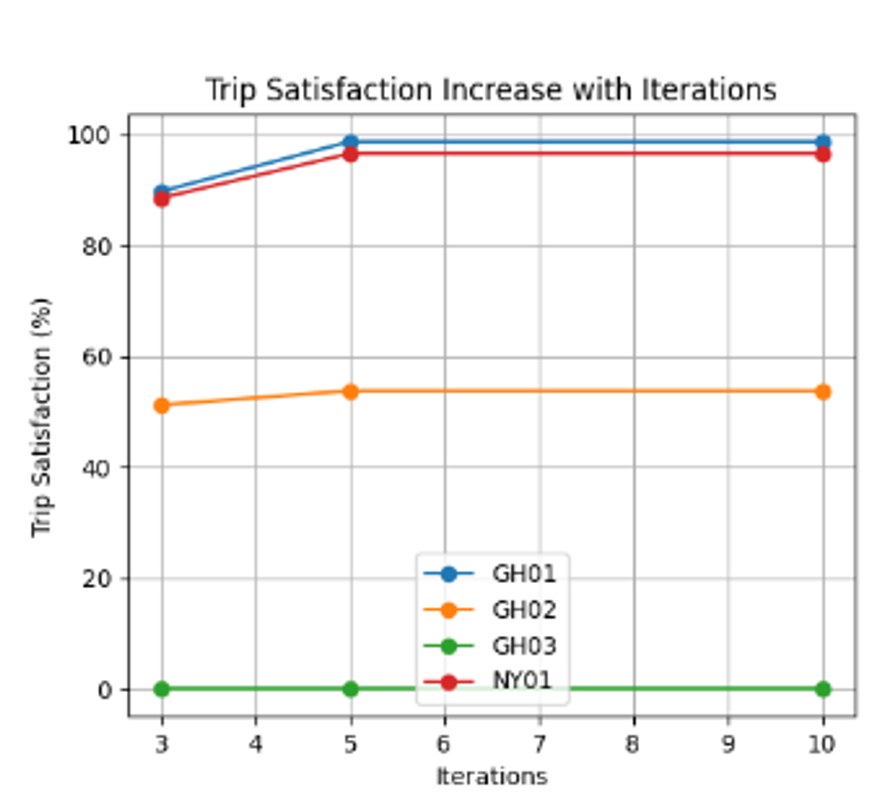
\includegraphics[scale=0.3]{Crest/Images/iterations.png}
  \caption{Number of Trips being Served over Iterations}
  \label{fig:iterations}
  \vspace{-0.1cm}
\end{figure}

\begin{figure}[h]
  \vspace{-0.2cm}
  \centering
  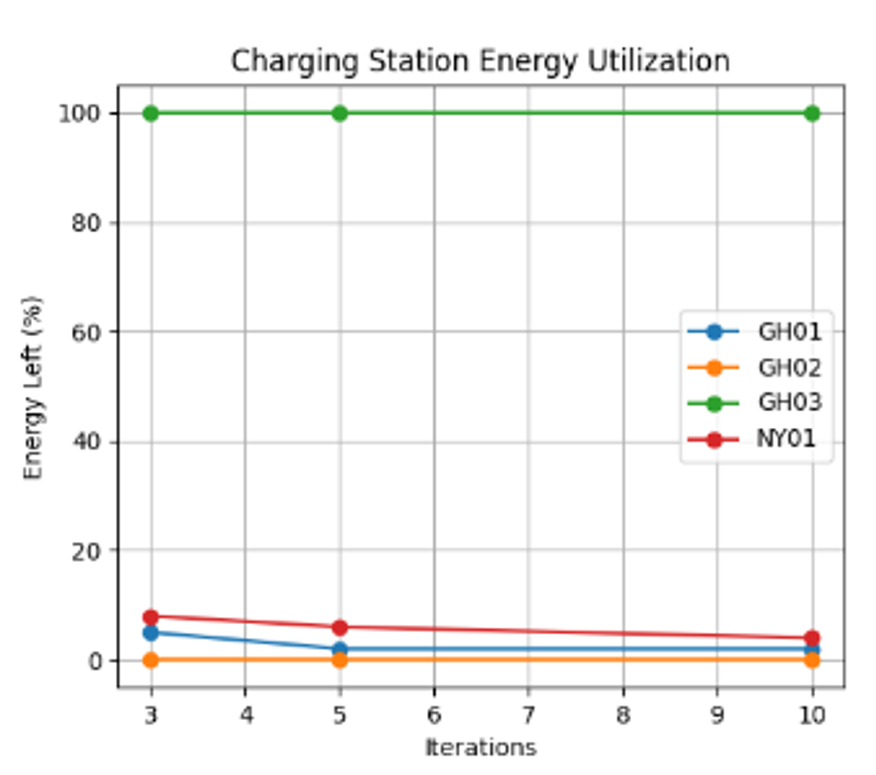
\includegraphics[scale=0.3]{Crest/Images/energy_charging_utilise.png}
  \caption{Energy Utilisation Efficiency}
  \label{fig:energy_charging_utilise}
  \vspace{-0.1cm}
\end{figure}


\begin{table}[htbp]
\caption{Improvement(\%) of Trips Served over Iterations}
\begin{center}
\begin{tabular}{|c|c|c|c|}
\hline
\textbf{Dataset} & \textbf{ Iterations} & \textbf{Improvement (\%)} & \textbf{Time (mins)} \\
\hline
GH01 & 3 & 8 & 7 \\
GH02 & 3 & 2 & 7 \\
GH03 & 3 & 0 & 2 \\
NY01 & 3 & 2.5 & 7 \\
GH01 & 5 & 10 & 10 \\
GH02 & 5 & 2 & 10 \\
GH03 & 5 & 0 & 2 \\
NY01 & 5 & 8 & 12 \\
GH01 & 10 & 10 & 10 \\
GH02 & 10 & 2 & 12 \\
GH03 & 10 & 0 & 2 \\
NY01 & 10 & 8 & 20 \\
\hline
\end{tabular}
\label{tab:trip_satisfaction}
\end{center}
\end{table}



\subsection{Charging Station Energy Utilisation}
Each SEC consists of a charging station with limited energy availability, denoted by the energy factor, which was efficiently managed by the algorithm. The number of times an AEV charged at a CS varied depending upon the initial trip allocation of the AEV and the reward procurement. 

CSs located near regions with high trip density became more in demand, as they offered shorter detours for AEVs with low battery levels. Furthermore, CSs positioned close to the boundaries between SECs experienced higher usage, as inter-SEC trips leveraged nearby charging infrastructure to minimise downtime. For instance, in the Hashcode dataset, the energy of each CS was utilised effectively, contributing to a higher number of TPs being served.

A more detailed analysis of spatial charging station demand patterns is provided in the following sections of this chapter.

Figure \ref{fig:avg_charges} shows the average number of charges per EV at different battery capacities for one of the Hashcode dataset instances (GH01). The x-axis represents the battery capacity, while the y-axis shows the average number of charges required. Higher battery capacities result in fewer charges, indicating more efficient energy use.
\begin{figure}[h]
  \vspace{-0.2cm}
  \centering
  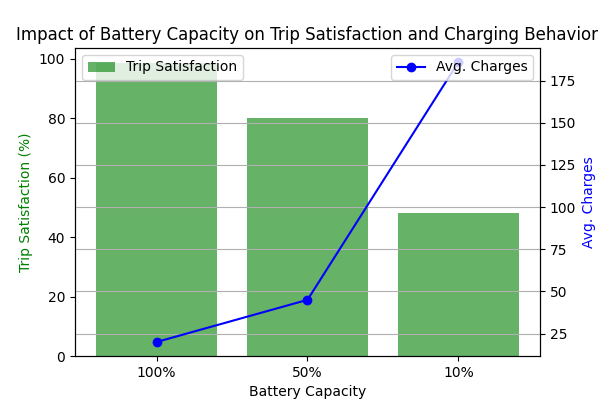
\includegraphics[scale=0.40]{Crest/Images/tripsatisfied_vs_battery.png}
  \caption{Impact of battery capacity on charging behavior}
  \label{fig:avg_charges}
  \vspace{-0.1cm}
\end{figure}

Table~\ref{tab:energy_utilization_tab} provides detailed results for the charging station energy utilisation across different datasets and iterations. The average number of charges per AEV and the remaining energy percentage at each SEC after the simulation is completed. 
\begin{table}[h]
\caption{Charging Station Energy Utilisation}
\begin{center}
\begin{tabular}{|c|c|c|c|c|}
\hline
\textbf{Dataset} & \textbf{SECs} & \textbf{Avg. Charges} & \textbf{Energy Left (\%)} & \textbf{Iterations} \\
\hline
GH01 & 16 & -- & 45 & 0 \\
GH01 & 16 & 15 & 5 & 3 \\
GH01 & 16 & 18 & 2 & 5 \\
GH01 & 16 & 20 & 2 & 10 \\
NY01 & 16 & -- & 50 & 0 \\
NY01 & 16 & 35 & 8 & 3 \\
NY01 & 16 & 45 & 6 & 5 \\
NY01 & 16 & 50 & 4 & 10 \\
\hline
\end{tabular}
\label{tab:energy_utilization_tab}
\end{center}
\end{table}


Before applying the charging scheduler (i.e., at 0 iterations), a substantial portion of energy remained unused --- approximately 45\% for GH01 and 50\% for NY01. After integrating the charging scheduler and running the iterative optimisation, the remaining total energy dropped significantly to as low as 2--4\%, reflecting highly efficient resource management. It is important to clarify here that the objective of the proposed charging scheduler is not to maximise energy consumption per se, but to maximise the number of trip petitions served while operating within the available renewable energy constraints.These results clearly demonstrate the impact and effectiveness of the charging scheduling algorithm in maximising the use of available renewable energy resources.


\subsection{Impact of Battery Capacity on Trip Served and Charging Behavior}

The impact of different battery capacities on trips served and charging behavior is significant. Table~\ref{tab:battery_capacity} summarises the performance across different battery capacities. AEVs with higher battery capacities required fewer charging sessions, leading to higher trip service rates. Conversely, AEVs with lower battery capacities needed to charge much more frequently, which disrupted their schedules and reduced the overall number of trips served.

\begin{table}[htbp]
\caption{Impact of Battery Capacity}
\begin{center}
\begin{tabular}{|c|c|c|c|}
\hline
\textbf{Data} & \textbf{Battery} & \textbf{Trips Served (\%)} & \textbf{Avg. Re-Charges/AEV} \\
\hline
GH01 & 100 & 98.66 & 20 \\
GH01 & 50 & 80.00 & 45 \\
GH01 & 10 & 48.00 & 186 \\
NY01 & 100 & 98.66 & 256 \\
NY01 & 50 & 80.00 & 505 \\
NY01 & 10 & 48.00 & 1290 \\
\hline
\end{tabular}
\label{tab:battery_capacity}
\end{center}
\end{table}

It is important to note that the last column represents the \textit{average number of re-charges per AEV} across the entire simulation horizon. The high values observed for lower battery capacities (e.g., 45 recharges per AEV for a battery capacity of 50) suggest that such capacities are not practical for real-world operations, as they would require vehicles to spend a significant portion of time charging rather than serving passengers.

Moreover, an additional comparison was made between the percentage of TPs served with and without charging infrastructure for different battery capacities. Without charging infrastructure, the trip service rate significantly drops, particularly for lower battery capacities. For instance, in GH01, a battery capacity of 50 served only around 42\% of trips without charging infrastructure, compared to 80\% with charging infrastructure. This highlights the critical role that the charging scheduling mechanism plays in maintaining service continuity, especially for fleets equipped with mid-sized or small battery AEVs.

\subsection{Impact of Rewards on Trip Served}

Table~\ref{tab:rewards} shows that when AEVs are given rewards for serving TPs from neighbouring SECs, the overall number of trips served increases dramatically. This is because AEVs that serve neighbouring SECs are allowed to recharge at nearby CSs, rather than returning to their home SEC for recharging. By leveraging the rewards accumulated, AEVs can optimise their routes more efficiently, significantly reducing downtime and enabling them to serve more TPs within the same time horizon.

\begin{table}[htbp]
\caption{Impact of Trip Served Reward}
\begin{center}
\begin{tabular}{|c|c|c|}
\hline
\textbf{Dataset} & \textbf{AEV Type} & \textbf{Trip Served (\%)} \\
\hline
GH01 & With Rewards & 98.66 \\
GH01 & Without Rewards & 39.69 \\
\hline
NY01 & With Rewards & 96.5 \\
NY01 & Without Rewards & 53.2 \\
\hline
\end{tabular}
\label{tab:rewards}
\end{center}
\end{table}

The improvement observed in GH01, from 39.69\% to 98.66\%, highlights the critical role that the reward mechanism plays in enhancing the efficiency and scalability of the ride-sharing system. Without rewards, AEVs are restricted to charging at their own SEC's stations, resulting in longer detours and increased idle time between trips. This leads to a large number of TPs being missed.

To further illustrate this impact, an analysis of the re-charging patterns in GH01 is conducted. Without rewards, AEVs in GH01 performed an average of 6.8 re-charges per AEV, with an average detour distance of 4.3 grid units to reach their home CSs. With rewards enabled, the average number of re-charges per AEV increased slightly to 7.5, but the average detour distance decreased sharply to 1.2 grid units. This reduction in detour distance enabled AEVs to minimise downtime, remain within high-demand areas, and rapidly serve subsequent TPs.

Thus, the reward mechanism not only increases the number of trips served but also improves spatial efficiency, allowing AEVs to remain operationally active for longer durations without being bottlenecked by long return trips to home CSs. This dynamic significantly contributes to the near-doubling of service rates observed in GH01 and NY01.

\subsection{Impact of Full Charge vs. Partial Charge}

As shown in Figure~\ref{fig:battery} and Table~\ref{tab:charging_strategy}, the strategy of fully charging AEVs, as opposed to releasing them after partial charges, was evaluated. Fully charged AEVs demonstrated a higher number of trips served and reduced the need for frequent recharges, whereas partially charged AEVs needed to return to CSs more often.

\begin{table}[h]
\caption{Impact of Charging Strategy on Number of Trips being Served}
\begin{center}
\begin{tabular}{|c|c|c|}
\hline
\textbf{Dataset} & \textbf{Charging Strategy} & \textbf{Trip Served (\%)} \\
\hline
GH01 & Full Charge & 98.66 \\
GH01 & Half Charge & 86.5 \\
GH01 & 70\% Charge & 90.0 \\
NY01 & Full Charge & 96.5 \\
NY01 & Half Charge & 80.8 \\
NY01 & 70\% Charge & 88.0 \\
\hline
\end{tabular}
\label{tab:charging_strategy}
\end{center}
\end{table}

\begin{figure}[h]
  \vspace{-0.2cm}
  \centering
  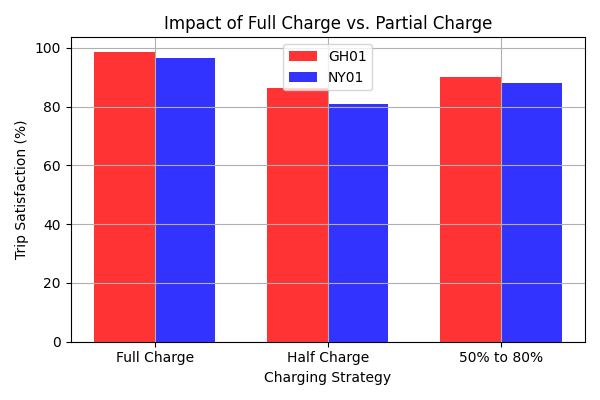
\includegraphics[scale=0.40]{Crest/Images/batery_capacitty.png}
  \caption{Impact of Charging Strategy}
  \label{fig:battery}
  \vspace{-0.1cm}
\end{figure}

These results suggest that, in general, it is more beneficial for AEVs to perform a full charge. Although full charging requires a longer stay at CSs — potentially causing AEVs to miss immediate trip opportunities — the overall system efficiency improves because vehicles can serve multiple trips consecutively without frequent interruptions for recharging.

However, this finding must be interpreted carefully in the context of the implemented \textit{eviction policy}. The eviction policy allows AEVs with higher potential (i.e., higher future trip value) to displace lower-priority AEVs from CSs. By design, eviction prevents the evicted AEVs from completing a full charge, forcing them to operate with partial battery levels.

This introduces a trade-off: while full charging is ideal for maximising the autonomy and service potential of AEVs, the eviction mechanism ensures that the most strategically important AEVs have access to charging infrastructure when needed. As a result, the system balances between:
\begin{itemize}
    \item Prioritising full charges for efficiency.
    \item Allowing strategic partial charges when necessary to maximise overall trip satisfaction.
\end{itemize}

In summary, full charging is preferable when possible, but the intelligent eviction policy ensures that the charging infrastructure remains dynamically optimised for the greater good of the entire system.

\section{Comparison with Baseline Algorithms}
\label{sec:baseline_comparison}

This section assesses the performance of the proposed charging scheduling solution approach against two baseline algorithms: First-Come, First-Served (FCFS) and Random Allocation. 

Two baselines are implemented:
\begin{itemize}
    \item \textbf{First-Come, First-Served (FCFS)}: In this algorithm, TPs are assigned to AEVs based on the order in which they arrive in the simulation. For each TP, the first available EV with enough battery and capacity is assigned to serve it.
  
    \item \textbf{Random Allocation}: In this algorithm, TPs are assigned to AEVs randomly, without considering their current battery capacity, their proximity to available CSs or their available energy.  
\end{itemize}

\subsection{FCFS Algorithm}

In Algorithm 6, the function \textit{FCFS\_Allocate} iterates over all TPs and tries to assign the first available AEV that can serve the TP. It checks for enough battery and capacity before assigning the TP.
The function\textit{ FCFS\_Charging} checks the battery levels of AEVs and sends those below a certain threshold  $\beta$  to the nearest charging station. No priority aspects are applied to the charging decisions.
\begin{algorithm}
\caption{First-Come, First-Served (FCFS) Algorithm}
\begin{algorithmic}
\Function{FCFS\_Allocate}{$T$, $E$, $Alloc$, $Sched$}
    \For{$t \in T$} \Comment{Iterate through all TPs}
        \For{$e \in E$} \Comment{Check each AEV}
            \If{$e$ can serve $t$} \Comment{AEV must have enough capacity and battery}
                \State $Alloc[t] \gets e$
                \State $Sched[e] \gets \text{update schedule with trip } t$
                \State \textbf{break}
            \EndIf
        \EndFor
    \EndFor
\EndFunction

\Function{FCFS\_Charging}{$E$, $CS$, $\beta$}
    \For{$e \in E$} \Comment{Check each AEV}
        \If{$e_{bc} \leq \beta$} \Comment{Battery below threshold}
            \State Send $e$ to nearest available charging station $cs$
        \EndIf
    \EndFor
\EndFunction
\end{algorithmic}
\end{algorithm}


\subsection{Random Allocation Algorithm}
  
In Algorithm 7, the function \textit{Random\_Allocate} randomly selects an AEV for each TP. It assigns the trip to the AEV if it has enough capacity and battery. If no suitable AEV is found, the TP is skipped.
The function \textit{Random\_Charging} sends AEVs with battery levels below the threshold  $\beta$ to a randomly selected charging station, leading to potentially inefficient energy utilisation.
\begin{algorithm}
\caption{Random Allocation Algorithm}
\begin{algorithmic}
\Function{Random\_Allocate}{$T$, $E$, $Alloc$, $Sched$}
    \For{$t \in T$} \Comment{Iterate through all TPs}
        \State $e \gets \text{Random AEV from } E$ \Comment{Randomly select an AEV}
        \If{$e$ can serve $t$} \Comment{AEV must have enough capacity and battery}
            \State $Alloc[t] \gets e$
            \State $Sched[e] \gets \text{update schedule with trip } t$
        \Else
            \State \text{Skip $t$ if no suitable AEV is available}
        \EndIf
    \EndFor
\EndFunction

\Function{Random\_Charging}{$E$, $CS$, $\beta$}
    \For{$e \in E$} \Comment{Check each AEV}
        \If{$e_{bc} \leq \beta$} \Comment{Battery below threshold}
            \State Send $e$ to a randomly selected charging station $cs$
        \EndIf
    \EndFor
\EndFunction
\end{algorithmic}
\end{algorithm}

As opposed to the two aforementioned algorithms, the proposed solution approach of Section 5.2 takes into account a variety of criteria, including trip weight, energy levels, accessibility to CSs, and future trip potential. It automatically modifies trip allocation and charging schedules to maximise trip served and energy efficiency. It includes a reward scheme in which AEVs are compensated for serving TPs from neighbouring SECs. It employs an iterative technique to fine-tuning both trip distribution and charging schedules, with the goal of achieving an optimal solution that maximises trips provided while remaining energy efficient.

The two baseline algorithms are evaluated under the same instances described in Section 5.3. The results are compared in terms of trip satisfaction, energy efficiency, and runtime performance.

\begin{enumerate}
    \item \textbf{Number of Trips Served}: This metric reflects the efficiency of the algorithms in serving TPs. A higher number of trips served indicates better service quality.

    \item \textbf{Energy Utilisation at CSs}: This metric measures how well the algorithms handle energy resources at CSs It calculates the percentage of available energy spent by AEVs when charging.

    \item \textbf{Computational Efficiency (Runtime)}: This metric measures the time taken by each algorithm to process the TPs and schedule AEVs. It reflects the scalability and computational complexity of the algorithms.
\end{enumerate}


\subsection{Analysis}
The results of the experiment are summarised in Tables \ref{tab:trips_served}, \ref{tab:energy_utilization}, and \ref{tab:runtime}. Figures \ref{fig:trips_served}, \ref{fig:energy_utilization} and \ref{fig:run_time} provide visual comparisons of the performance of the algorithms

\begin{table}[htbp]
\caption{Number of Trips Served by Each Algorithm}
\centering
\begin{tabular}{|c|c|c|c|}
\hline
\textbf{Dataset} & \textbf{Proposed Algorithm} & \textbf{FCFS} & \textbf{Random Allocation} \\
\hline
Hashcode & 98.66\% & 89.69\% & 76.34\% \\
NYC & 96.50\% & 85.23\% & 72.11\% \\
\hline
\end{tabular}
\label{tab:trips_served}
\end{table}

\begin{table}[htbp]
\caption{Energy Utilisation at CSs}
\centering
\begin{tabular}{|c|c|c|c|}
\hline
\textbf{Dataset} & \textbf{Proposed Algorithm} & \textbf{FCFS} & \textbf{Random Allocation} \\
\hline
Hashcode & 95.12\% & 83.45\% & 72.89\% \\
NYC & 94.23\% & 81.56\% & 70.34\% \\
\hline
\end{tabular}
\label{tab:energy_utilization}
\end{table}

\begin{table}[htbp]
\caption{Runtime (in Minutes) of Each Algorithm}
\centering
\begin{tabular}{|c|c|c|c|}
\hline
\textbf{Dataset} & \textbf{Proposed Algorithm} & \textbf{FCFS} & \textbf{Random Allocation} \\
\hline
Hashcode & 10 & 8 & 7 \\
NYC & 20 & 18 & 15 \\
\hline
\end{tabular}
\label{tab:runtime}
\end{table}

\begin{figure}[htbp]
\centering
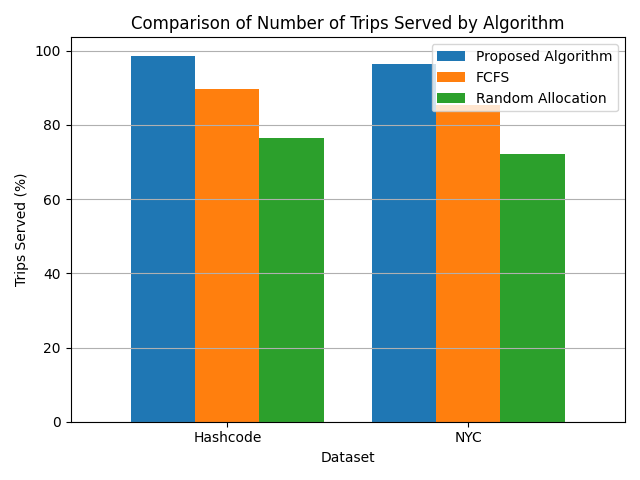
\includegraphics[scale=0.55]{Crest/Images/trips_served_comparison.png}
\caption{Number of Trips Served by Each Algorithm}
\label{fig:trips_served}
\end{figure}

\begin{figure}[htbp]
\centering
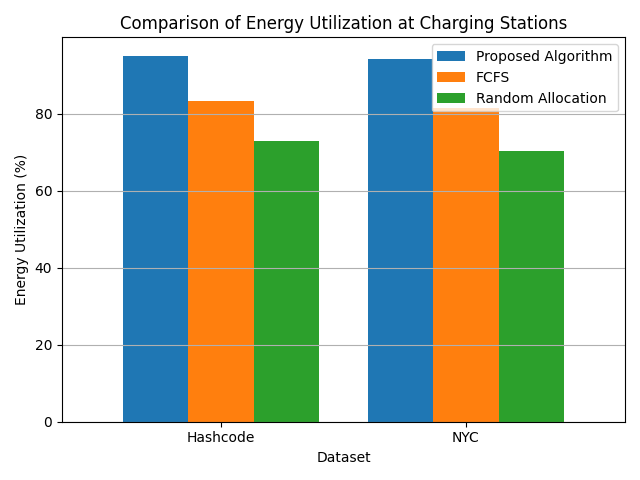
\includegraphics[scale=0.55]{Crest/Images/energy_utilization_comparison.png}
\caption{Energy Utilization at CSs}
\label{fig:energy_utilization}
\end{figure}

\begin{figure}[htbp]
\centering
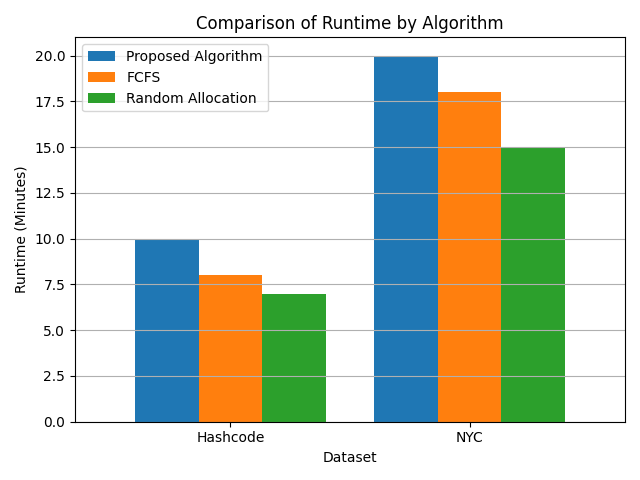
\includegraphics[scale=0.55]{Crest/Images/runtime_comparison.png}
\caption{Energy Utilization at CSs}
\label{fig:run_time}
\end{figure}

As shown in Table \ref{tab:trips_served} and Figure \ref{fig:trips_served}, the suggested method consistently outperforms both the FCFS and Random Allocation algorithms in terms of the amount of TPs being served. In the Hashcode dataset, the proposed approach served 98.66\% of TPs, while FCFS served 89.69\% and Random Allocation served just 76.34\%. A similar pattern was identified in the NYC sample.

In terms of energy utilisation (Table \ref{tab:energy_utilization} and Figure \ref{fig:energy_utilization}), the proposed algorithm demonstrated better energy management at CSs, utilising 95.12\% of available energy in the Hashcode dataset, compared to 83.45\% for FCFS and 72.89\% for Random Allocation. This pattern was consistent across both datasets.

As indicated in Table \ref{tab:runtime} and Figure \ref{fig:run_time}, the suggested method had a slightly higher runtime compared to the baseline algorithms, due to the difficulty of optimising the charging schedules and trip allocations. However, the increased runtime is offset by a large gain in trips served and energy efficiency.

\section{Impact of Charging Speed (Fast Charging vs. Slow Charging)}
\label{sec:charging_speed}

This section evaluates the performance of the ride-sharing system when different charging rates (fast vs. slow) are available at distinct charging stations. The analysis considers the number of TPs served, and the congestion at charging stations. 

Two types of charging rates are considered for the CSs:
\begin{itemize}
    \item \textbf{Fast Chargers}: High-speed charging stations,  capable of recharging AEVs at a rate of 15 kWh per unit time.
    \item \textbf{Slow Chargers}: Low-speed charging stations, capable of re-charging AEVs at a rate of 5 kWh per hour unit time.
\end{itemize}

The results are compared in terms of the following metrics:
\begin{itemize}
    \item \textbf{Number of Trips Served}: The total number of trips petitions served by the system under fast and slow charging configurations.
    \item \textbf{Average Waiting Time at Charging Stations}: The average time AEVs spend waiting to access a charging station, indicating congestion levels.
\end{itemize}

The simulation is run on the same Google HashCode and NYC instances as in section 5.4.

\subsection{Analysis}
Tables \ref{tab:trips_served_charging_speed}, \ref{tab:waiting_time}, and Figures \ref{fig:trips_served_charging_speed},  \ref{fig:waiting_time} provide the results.

\begin{table}[h]
\caption{Number of TPs Served under Different Charging Speeds}
\centering
\begin{tabular}{|c|c|c|}
\hline
\textbf{Dataset} & \textbf{50\% Fast / 50\% Slow Chargers} & \textbf{100\% Slow Chargers} \\
\hline
Google Hashcode & 98.66\% & 89.12\% \\
NYC & 96.50\% & 84.25\% \\
\hline
\end{tabular}
\label{tab:trips_served_charging_speed}
\end{table}

\begin{table}[h]
\caption{Average Waiting Time at Charging Stations (in Minutes)}
\centering
\begin{tabular}{|c|c|c|}
\hline
\textbf{Dataset} & \textbf{50\% Fast / 50\% Slow Chargers} & \textbf{100\% Slow Chargers} \\
\hline
Google Hashcode & 5.2 & 12.8 \\
NYC & 7.5 & 16.2 \\
\hline
\end{tabular}
\label{tab:waiting_time}
\end{table}

\begin{figure}[h]
\centering
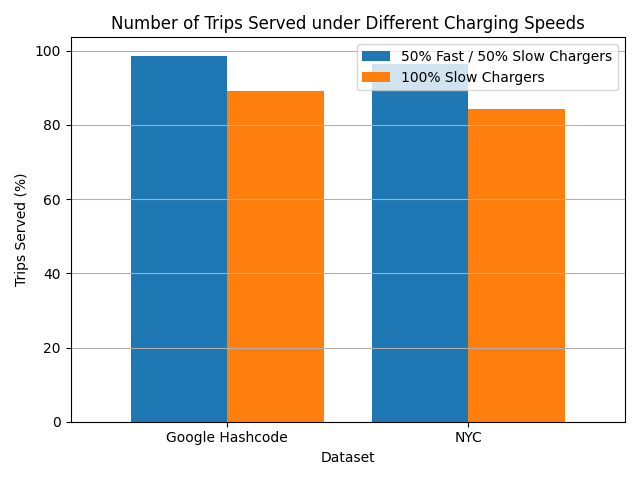
\includegraphics[scale=0.55]{Crest/Images/trips_served_charging_speed.png}
\caption{Number of Trips Served under Different Charging Speeds}
\label{fig:trips_served_charging_speed}
\end{figure}

\begin{figure}[h]
\centering
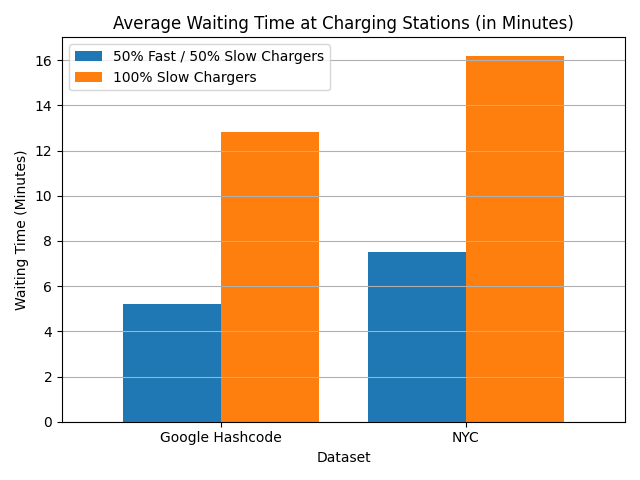
\includegraphics[scale=0.55]{Crest/Images/waiting_time_charging_speed.png}
\caption{Average Waiting Time at Charging Stations (in Minutes)}
\label{fig:waiting_time}
\end{figure}

Table \ref{tab:trips_served_charging_speed} and Figure \ref{fig:trips_served_charging_speed} indicate that using 50\% fast chargers results in considerably more trips served compared to 100\% slow chargers. In the Google Hashcode dataset, the system serves 98.66\% of TPs with fast chargers, and only 89.12\% with slow chargers. A similar tendency is seen in the NYC dataset.

Fast chargers reduce the average waiting time at charging stations significantly (Table \ref{tab:waiting_time} and Figure \ref{fig:waiting_time}). According to the Google Hashcode dataset, charging stations with 50\% fast chargers have an average waiting time of 5.2 time units, whereas 100\% slow chargers take 12.8 time units. Similar trends are seen in the NYC dataset.

\section{Impact of Renewable Energy Availability at Charging Stations}
\label{sec:renewable_energy}

This section assesses how fluctuations in availability of RES impact AEV charging schedules and overall amount of TPs being served.

The experiment models RES fluctuations at charging stations based on the following two scenarios:
\begin{itemize}
    \item \textbf{Scenario 1: Solar Power Availability} – Solar energy is available only during daytime, with energy production peaking around noon and no energy available during nighttime.
    \item \textbf{Scenario 2: Wind Energy Variability} – Wind energy fluctuates throughout the day, with varying energy availability depending on weather conditions.
\end{itemize}

The following metrics are analysed:

\begin{itemize}
    \item \textbf{Charging Station Utilisation}: The percentage of time charging stations are occupied and actively charging AEVs under varying energy availability.
    \item \textbf{Number of Trips Served}: The total number of TPs successfully served under each energy scenario.
    \item \textbf{Frequency of Charging Delays}: The number of discrete instances where AEVs experience delays in charging due to limited energy availability at CSs.
\end{itemize}

Tables \ref{tab:charging_utilization}, \ref{tab:trips_served_renewable}, and \ref{tab:charging_delays_renewable} summarize the results, and Figures \ref{fig:charging_utilization}, \ref{fig:trips_served_renewable}, and \ref{fig:charging_delays_renewable} provide visual comparisons.

\begin{table}[htbp]
\caption{Charging Station Utilisation under Different Energy Scenarios}
\centering
\begin{tabular}{|c|c|c|c|}
\hline
\textbf{Dataset} & \textbf{Baseline (Constant Energy)} & \textbf{Solar Power} & \textbf{Wind Power} \\
\hline
Google Hashcode & 85.5\% & 65.2\% & 72.1\% \\
NYC & 90.1\% & 70.3\% & 78.5\% \\
\hline
\end{tabular}
\label{tab:charging_utilization}
\end{table}

\begin{table}[htbp]
\caption{Number of Trips Served with Varying Renewable Energy Availability}
\centering
\begin{tabular}{|c|c|c|c|}
\hline
\textbf{Dataset} & \textbf{Baseline (Constant Energy)} & \textbf{Solar Power} & \textbf{Wind Power} \\
\hline
Google Hashcode & 98.66\% & 85.12\% & 90.23\% \\
NYC & 96.50\% & 82.15\% & 88.05\% \\
\hline
\end{tabular}
\label{tab:trips_served_renewable}
\end{table}

\begin{table}[htbp]
\caption{Frequency of Charging Delays under Different Energy Scenarios}
\centering
\begin{tabular}{|c|c|c|c|}
\hline
\textbf{Dataset} & \textbf{Baseline (Constant Energy)} & \textbf{Solar Power} & \textbf{Wind Power} \\
\hline
Google Hashcode & 0 & 215 & 128 \\
NYC & 0 & 425 & 240 \\
\hline
\end{tabular}
\label{tab:charging_delays_renewable}
\end{table}

Table \ref{tab:charging_utilization} and Figure \ref{fig:charging_utilization} indicate a considerable decrease in charging station use during fluctuating energy conditions. Solar electricity, which is only available during the day, yields lower utilisation than the baseline situation. Wind power, albeit variable, provides more consistent availability than solar, resulting in higher utilisation.

\begin{figure}[htbp]
\centering
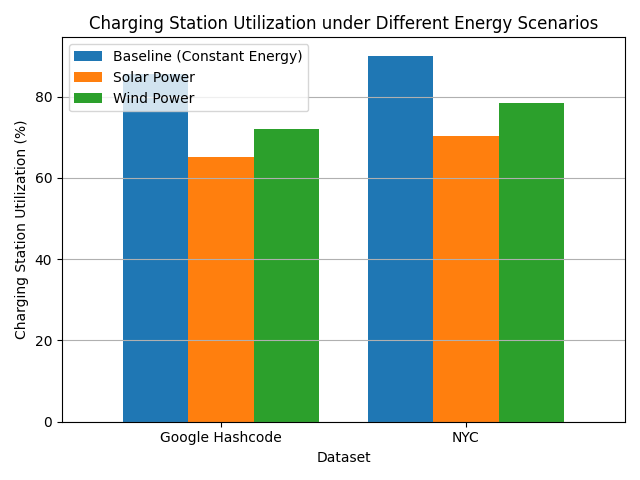
\includegraphics[scale=0.55]{Crest/Images/charging_utilization.png}
\caption{Charging Station Utilisation under Different Energy Scenarios}
\label{fig:charging_utilization}
\end{figure}

Table \ref{tab:trips_served_renewable} and Figure \ref{fig:trips_served_renewable} demonstrate that the number of trips served reduces as energy availability varies. Solar power has the highest impact, serving 85.12\% of TPs in the Google Hashcode dataset, compared to 98.66\% in the baseline. Wind power outperforms other kinds of energy due to its consistency.

\begin{figure}[htbp]
\centering
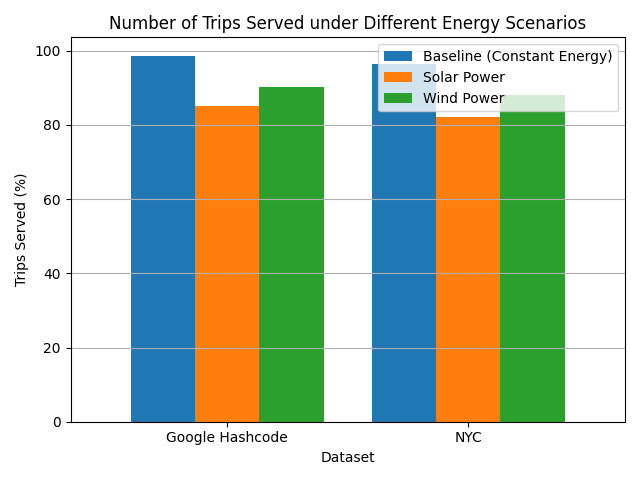
\includegraphics[scale=0.55]{Crest/Images/trips_served_renewable.png}
\caption{Number of Trips Served under Different Energy Scenarios}
\label{fig:trips_served_renewable}
\end{figure}

Table \ref{tab:charging_delays_renewable} and Figure \ref{fig:charging_delays_renewable} show that charging delays are common in both renewable energy situations. Solar electricity causes the most delays because of its limited availability at night.

\begin{figure}[htbp]
\centering
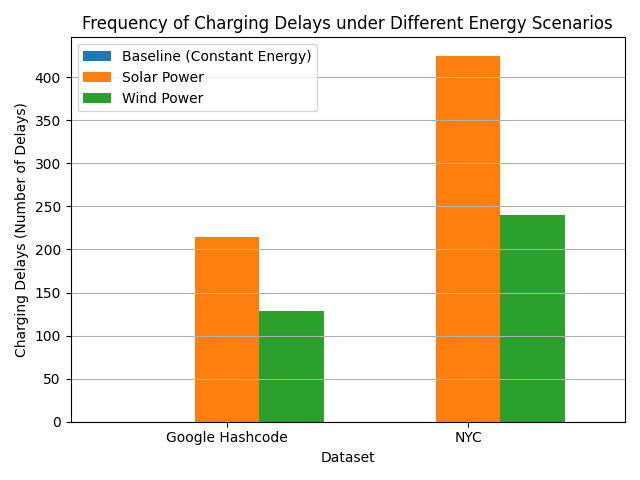
\includegraphics[scale=0.55]{Crest/Images/charging_delays_renewable.png}
\caption{Frequency of Charging Delays under Different Energy Scenarios}
\label{fig:charging_delays_renewable}
\end{figure}

The findings suggest that fluctuations in renewable energy have a major impact on the performance of the ride-sharing system. Solar energy, while sustainable, presents significant issues because to its limited availability at night, resulting in reduced charging station utilisation, fewer trips served, and longer charging delays. Wind power, while variable, provides more consistent energy supply and improves system performance. Incorporating energy storage technology or hybrid energy sources could help alleviate these effects.

\section{Impact of Varying Levels of Flexibility in TPs}
\label{sec:flexibility_trip_requests}

This section assesses how different levels of flexibility in trip pick-up and drop-off windows impact the capacity of the system to arrange trips and manage charging schedules. The relationship between flexibility and system efficiency, as well as how it affects the number of trips served, charging schedules, and energy use is examined.

The experiment simulates scenarios with varying levels of flexibility in TPs:
\begin{itemize}
    \item \textbf{Strict Flexibility}: Trips must be completed within a narrow time window, allowing minimal flexibility (e.g., 0.1 flexibility factor).
    \item \textbf{Moderate Flexibility}: Trip pick-up and drop-off windows are moderately flexible (e.g., 0.25 flexibility factor).
    \item \textbf{High Flexibility}: TPs are highly flexible, allowing significant leeway in pick-up and drop-off times (e.g., 0.5 flexibility factor).
\end{itemize}

The following key metrics are used for the evaluation:
\begin{itemize}
    \item \textbf{Percentage of Trips Served}: The proportion of TPs successfully allocated and completed under different flexibility levels.
    \item \textbf{Charging Station Utilisation}: The percentage of charging stations filled by AEVs at various levels of flexibility.
    \item \textbf{System Efficiency}: The relationship between trip flexibility and overall system efficiency, as determined by the energy consumed per trip and the total number of trips served.
\end{itemize}

% \subsection{Experimental Setup}
% The simulation is run on the following datasets:
% \begin{itemize}
%     \item \textbf{Google Hashcode Dataset}: 10,000 trip petitions and 400 AEVs.
%     \item \textbf{NYC Dataset}: 50,000 trip petitions and 1,000 AEVs.
% \end{itemize}

% Three levels of flexibility are simulated:
% \begin{enumerate}
%     \item \textbf{Strict Flexibility (5 min window)}: Very strict pick-up and drop-off time windows.
%     \item \textbf{Moderate Flexibility (15 min window)}: Moderate flexibility in time windows.
%     \item \textbf{High Flexibility (30 min window)}: High flexibility in pick-up and drop-off windows.
% \end{enumerate}

Tables \ref{tab:trips_served_flexibility}, \ref{tab:charging_utilization_flexibility}, and \ref{tab:system_efficiency_flexibility} provide a summary of the experiment output. Figures \ref{fig:trips_served_flexibility}, \ref{fig:charging_utilization_flexibility}, and \ref{fig:system_efficiency_flexibility} show visual comparisons.

\begin{table}[h]
\caption{Percentage of Trips Served under Different Flexibility Levels}
\centering
\begin{tabular}{|c|c|c|c|}
\hline
\textbf{Dataset} & \textbf{Strict} & \textbf{Moderate } & \textbf{High } \\
\hline
Google Hashcode & 78.9\% & 90.2\% & 98.1\% \\
NYC & 75.4\% & 88.5\% & 96.4\% \\
\hline
\end{tabular}
\label{tab:trips_served_flexibility}
\end{table}

\begin{table}[h]
\caption{Charging Station Utilisation under Different Flexibility Levels}
\centering
\begin{tabular}{|c|c|c|c|}
\hline
\textbf{Dataset} & \textbf{Strict} & \textbf{Moderate} & \textbf{High} \\
\hline
Google Hashcode & 72.3\% & 65.5\% & 59.8\% \\
NYC & 78.5\% & 68.7\% & 61.2\% \\
\hline
\end{tabular}
\label{tab:charging_utilization_flexibility}
\end{table}

\begin{table}[h]
\caption{System Efficiency under Different Flexibility Levels}
\centering
\begin{tabular}{|c|c|c|c|}
\hline
\textbf{Dataset} & \textbf{Strict} & \textbf{Moderate} & \textbf{High} \\
\hline
Google Hashcode & 1.5 units/trip & 1.2 units/trip & 1.0 units/trip \\
NYC & 1.6 units/trip & 1.3 units/trip & 1.1 units/trip \\
\hline
\end{tabular}
\label{tab:system_efficiency_flexibility}
\end{table}

Table \ref{tab:trips_served_flexibility} and Figure \ref{fig:trips_served_flexibility} show that as TPs become more flexible, the proportion of trips served rises. The Google Hashcode statistics shows that 98.1\% of TPs were served with high flexibility, whereas only 78.9\% were given with strict flexibility.

\begin{figure}[h]
\centering
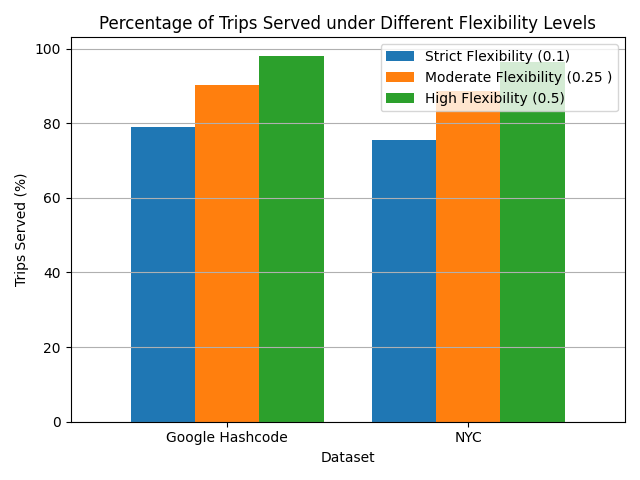
\includegraphics[scale=0.55]{Crest/Images/trips_served_flexibility.png}
\caption{Percentage of Trips Served under Different Flexibility Levels}
\label{fig:trips_served_flexibility}
\end{figure}

\begin{figure}[h]
\centering
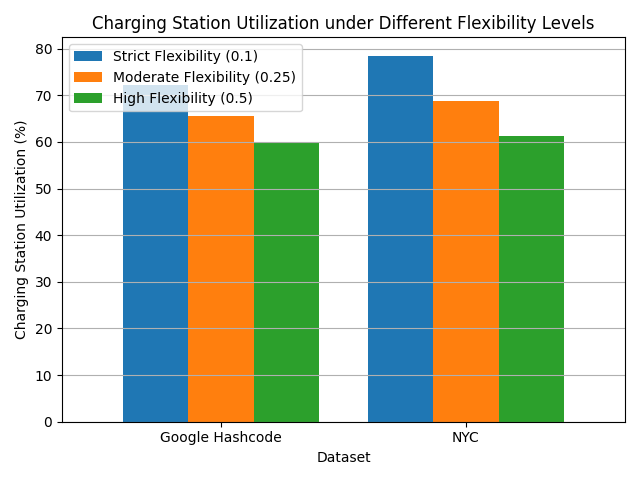
\includegraphics[scale=0.55]{Crest/Images/charging_utilization_flexibility.png}
\caption{Charging Station Utilization under Different Flexibility Levels}
\label{fig:charging_utilization_flexibility}
\end{figure}

\begin{figure}[h]
\centering
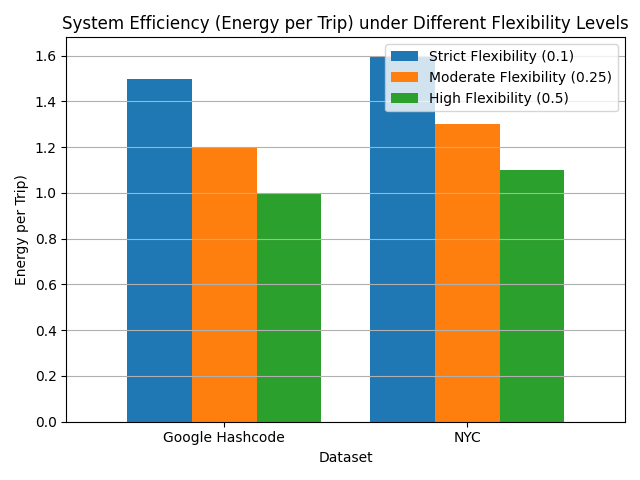
\includegraphics[scale=0.55]{Crest/Images/system_efficiency_flexibility.png}
\caption{System Efficiency (Energy per Trip) under Different Flexibility Levels}
\label{fig:system_efficiency_flexibility}
\end{figure}

Table \ref{tab:charging_utilization_flexibility} and Figure \ref{fig:charging_utilization_flexibility} show that charging station usage decreases as flexibility increases. This is because variable trip time windows enable more efficient scheduling of AEVs, resulting in less congestion at charging stations.

Table \ref{tab:system_efficiency_flexibility} and Figure \ref{fig:system_efficiency_flexibility} demonstrate that greater flexibility leads to higher system efficiency. The energy consumed per trip is lowered since AEVs may be better routed and timed with more flexible trip time slots, which results in lower energy consumption.

\section{Conclusions}
\label{sec:conclusions_and_future_work}

This chapter has presented the design, implementation, and evaluation of an reward-based, scalable charging scheduling algorithm for the carbon-neutral, community-based ride-sharing service. The model integrates multiple constraints, including energy usage, vehicle distribution, route planning, and charging station availability. The solution approach involves two key algorithms: a vehicle routing algorithm and a vehicle charging algorithm, which work in tandem to optimise the number of trips being served and energy efficiency.

The evaluation has been conducted using the same real-world datasets from Google Hashcode and NYC taxi services as per previous chapters. The proposed algorithm is designed to be flexible and adaptable to different urban environments by supporting a wide range of SECs, AEVs, TPs and CSs. 

The results demonstrate that the proposed scheduling algorithm significantly improves trip served and charging efficiency, with the system effectively handling large volumes of TPs and AEVs within a few minutes. The vehicle charging algorithm effectively meets the needs of urban transportation and sustainable energy management. By taking into account various constraints and rewards, it enhances the efficiency and reliability of the community-based ride-sharing service. The complete code can be accessed via GitHub \cite{rewardcharging}.

%As a final note, implementing a ride-sharing service that rewards users and operates without generating carbon emissions can help decrease the environmental impact of cities and encourage the adoption of sustainable transportation methods. The complete code can be accessed via GitHub \cite{rewardcharging}.